\documentclass[main.tex]{subfiles}
\begin{document}

\texttt{apt-cacher-ng} is a caching proxy for Debian/Ubuntu based package
manages. It is used to reduce network bandwidth while updating pacakges when a
network has a large number of clients.

\begin{figure}[H]
  \centering
  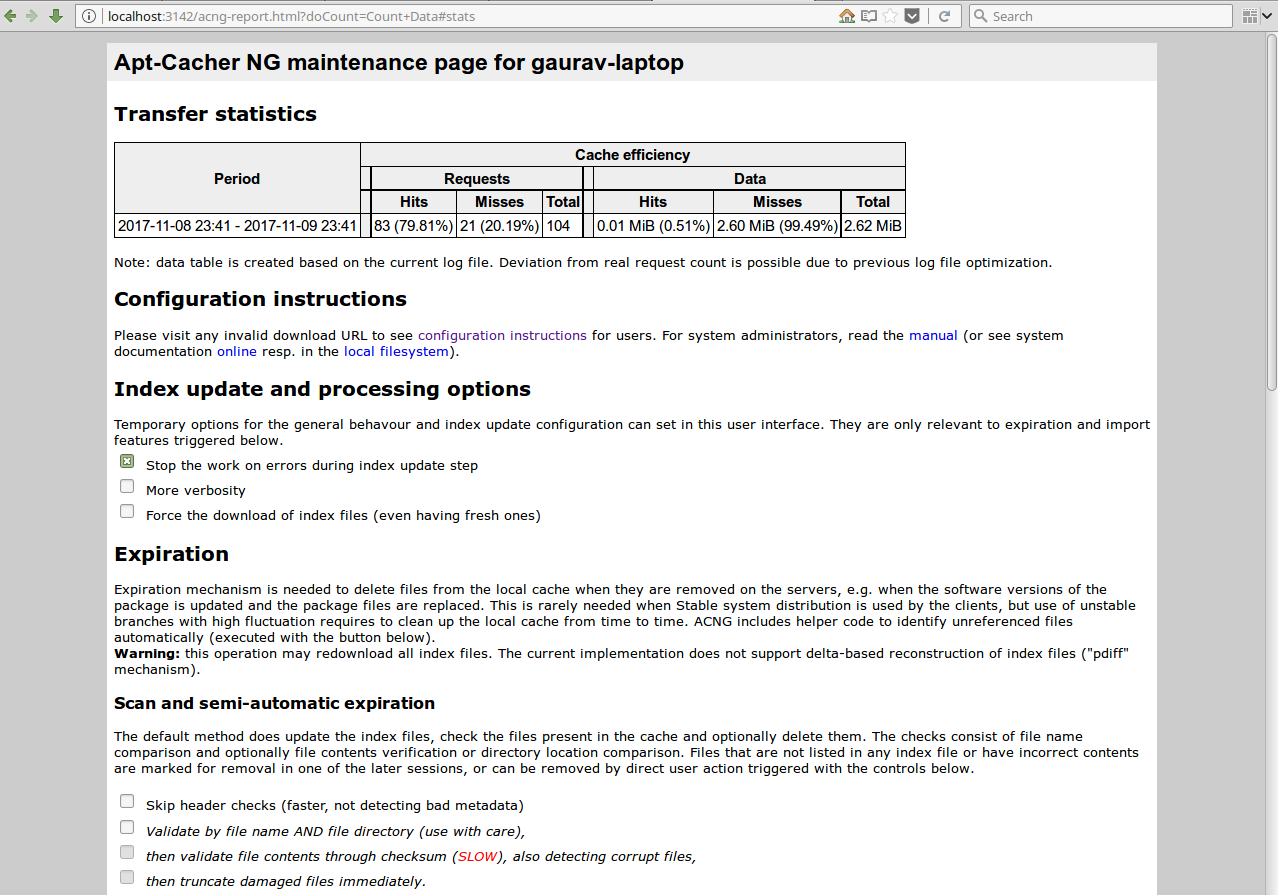
\includegraphics[width=\textwidth]{maint.png}
  \caption{Maintenance and statistics page for apt-cacher-ng}
\end{figure}

\begin{figure}[H]
  \centering
  
\includegraphics[width=\textwidth]{client_config.png}
  \caption{Minimal client configuration}
\end{figure}

\texttt{apt} can be configured to request pacakges through a proxy. Setting up
\texttt{apt-cacher-ng} as a proxy on the same machine can help during
development and Debian packaging when the same packages are needed to be
reinstalled many times.

\begin{figure}[H]
  \centering
  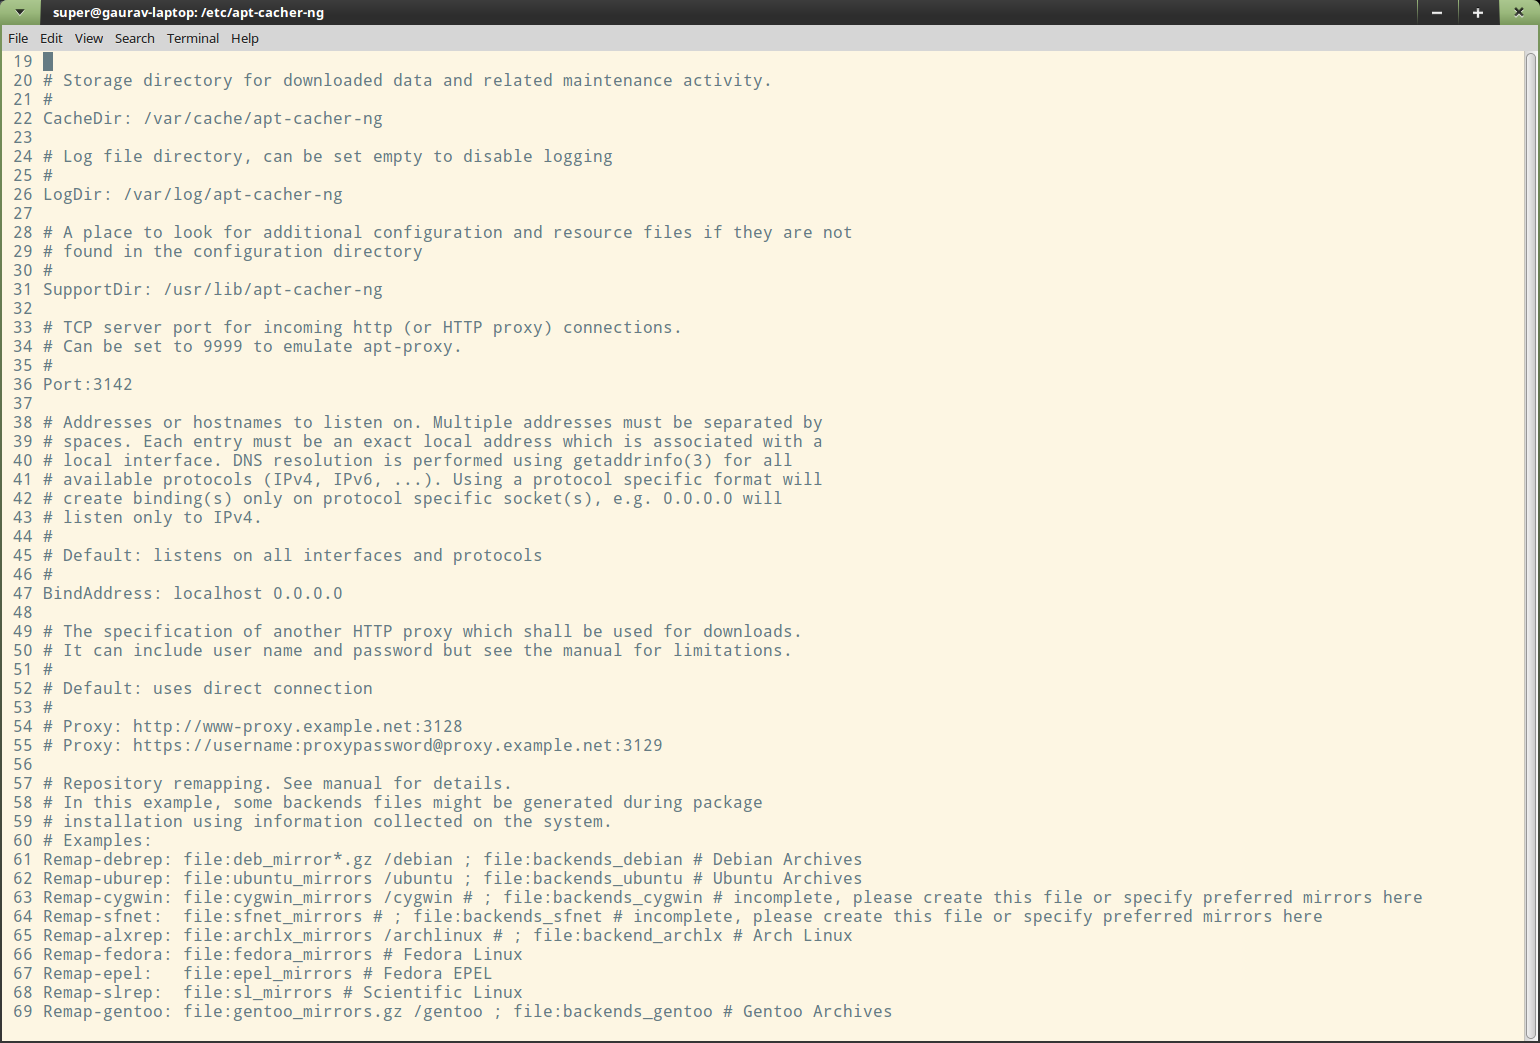
\includegraphics[width=\textwidth]{cache_conf.png}
  \caption{Server configuration}
\end{figure}

\end{document}
